\section{Implementation and Object-Oriented Principles}
\label{sec:implementation_oop}

This section delves into the implementation details of the system, with a specific focus on how the four fundamental principles of Object-Oriented Programming (OOP) \cite{Booch2007} were realized using the features of the C++ programming language \cite{Stroustrup2013}. The use of these principles was crucial for developing a system that is not only functional but also robust, modular, and maintainable.

\subsection{Encapsulation}
Encapsulation is the practice of bundling data and the methods that operate on that data into a single unit, while restricting direct access. This is achieved in C++ through access specifiers (`public`, `private`, `protected`).

In this project, all domain models enforce encapsulation. For example, the \texttt{User} class declares its attributes \texttt{userID} and \texttt{password} as \texttt{private}. Access from outside the class is only permitted through its public interface, protecting the object's internal state.

\begin{figure}[H]
	\centering
	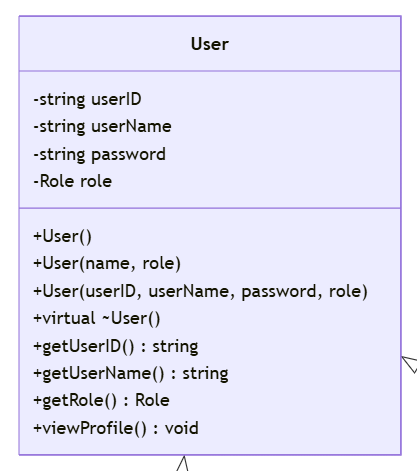
\includegraphics[width=0.5\textwidth]{figures/user_class_encap.png}
	\caption{UML Diagram for the User Class with Encapsulation.}
	\label{fig:user_class_encap}
\end{figure}

\subsection{Inheritance}
Inheritance allows a new class (subclass) to be based on an existing class (base class), promoting code reusability. C++ supports this directly through class derivation.

The system utilizes inheritance to model user types. The \texttt{Member} and \texttt{Librarian} classes both inherit publicly from the base \texttt{User} class. They acquire common attributes and functionalities while also implementing their own specialized methods.

\begin{figure}[H]
	\centering
	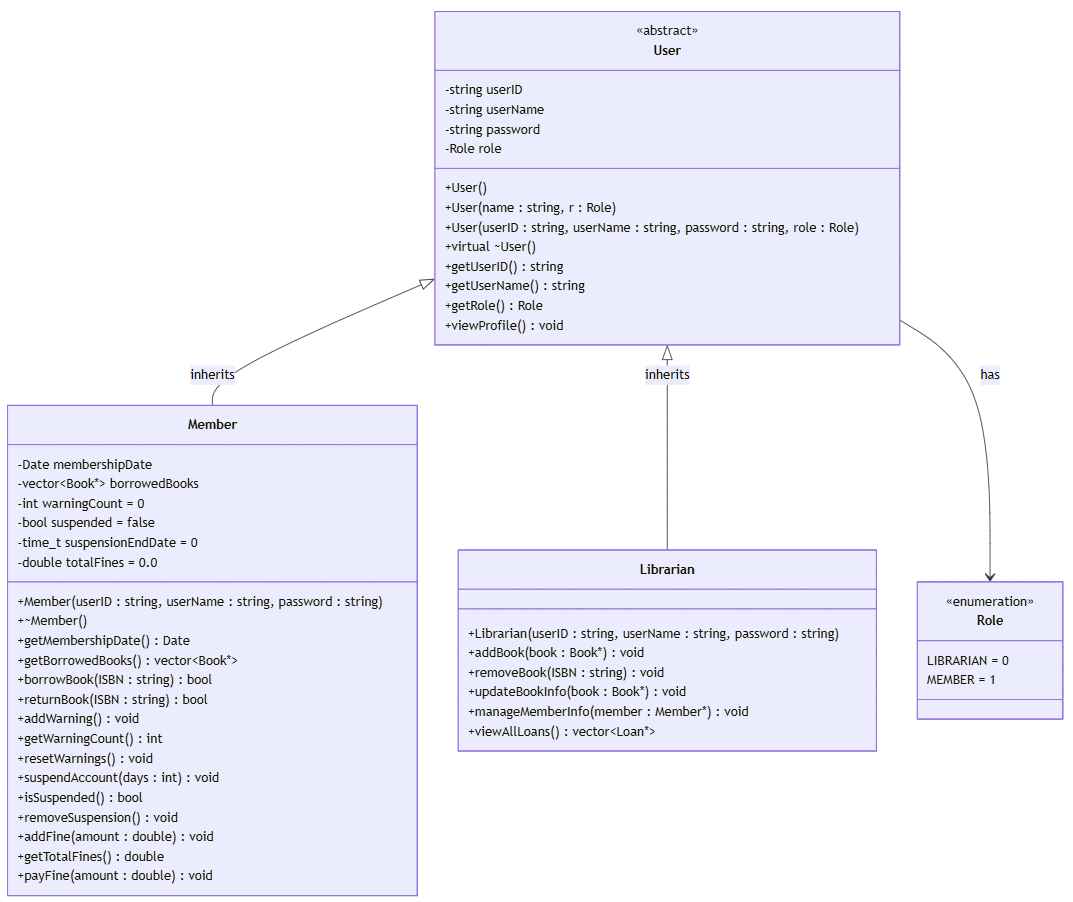
\includegraphics[width=1\textwidth]{figures/inheritance.png}
	\caption{UML Diagram for the User Class with Inheritance.}
	\label{fig:user_class_inheritance}
\end{figure}

\subsection{Polymorphism}
Polymorphism allows objects of different classes to be treated as objects of a common superclass. In C++, this is primarily achieved at runtime through \texttt{virtual} functions.

A clear example is the Strategy pattern implemented in the \texttt{SearchManager} class. The \texttt{SearchManager} contains a pointer to an \texttt{ISearchStrategy} interface and delegates search operations to concrete strategy implementations. When \texttt{search()} is called on the strategy pointer, C++'s dynamic dispatch mechanism ensures the correct overridden version (e.g., \texttt{TitleSearchStrategy}, \texttt{AuthorSearchStrategy}) is invoked at runtime, allowing the search behavior to be changed dynamically.

\begin{figure}[H]
	\centering
	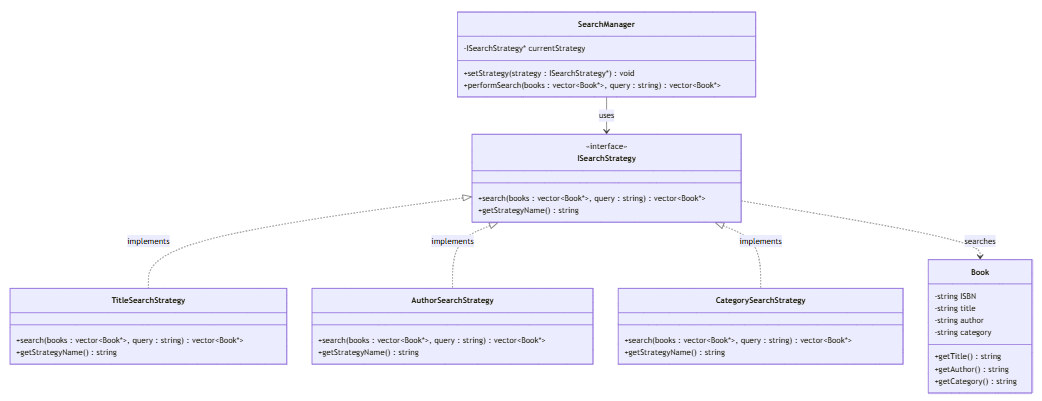
\includegraphics[width=1\textwidth]{figures/polymorphism.png}
	\caption{UML Diagram for Search Strategies with Polymorphism.}
	\label{fig:search_strategies_polymorphism}
\end{figure}

\subsection{Abstraction}
Abstraction involves hiding complex implementation details and exposing only essential functionalities. In C++, this is often achieved using abstract classes (classes with one or more pure virtual functions).

This principle is demonstrated through the Decorator pattern implementation. An abstract base class, \texttt{BookDecorator}, is defined with pure virtual functions that establish a contract for all concrete decorators. This abstraction allows clients to work with decorated books without knowing the specific decoration implementations, effectively hiding the complexity of feature additions while providing a unified interface.

\begin{figure}[H]
	\centering
	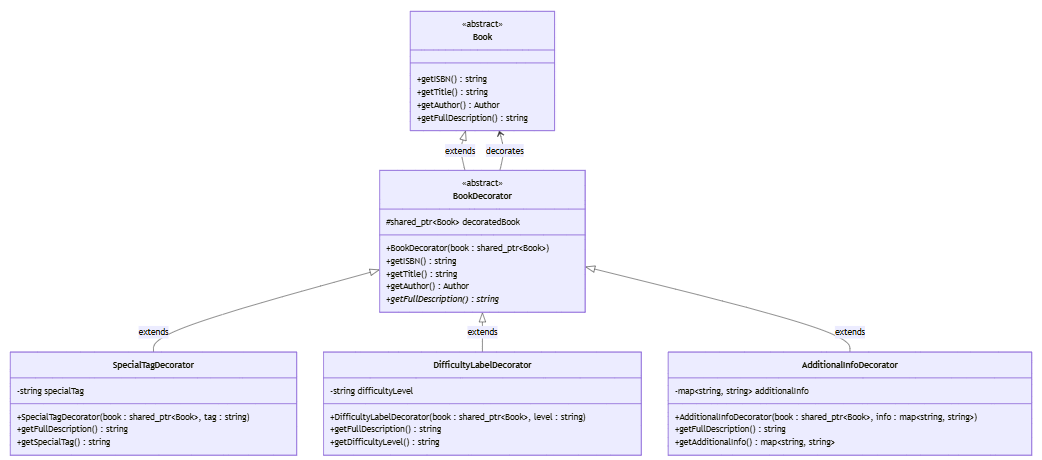
\includegraphics[width=1\textwidth]{figures/abstraction.png}
	\caption{UML Diagram for Book Decorator with Abstraction.}
	\label{fig:book_decorator_abstraction}
\end{figure}